%% %% %% %%
%%
%% Parte C de la práctica
%%
%% %% %% %%

\documentclass[../procedimientos.tex]{subfiles}
\graphicspath{{\subfix{../../images/}}}

\begin{document}
\clearpage
\subsection{Parte C}
\subsubsection*{Propuesta}
\begin{em}
  Se propone llevar a cabo el sistema planteado en la Sección 
  \ref{subs:previo} haciendo uso del lenguaje VHDL, en donde se tiene un 
  circuito \textbf{Desplazador-Rotador} que toma como entrada una palabra de 4 
  bits y devuelve otra palabra de 4 bits. Esto, con la finalidad de llevar a 
  la práctica el uso de los multiplexores y verificar el funcionamiento del 
  circuito.
\end{em}

\subsection*{Solución}
Tal como ya se plenteó anteriormente, la solución al problema (al menos de 
forma conceptual) se puede ver en la Figura \ref{fig:previo1}.

Para dar solución al problema, únicamente se requirieron implementar dos 
entidades. Por un lado, el multiplexor 4:1 (\textit{Mux4}); y por otro, el 
circuito Desplazador-Rotador que por en sí mismo representa la solución al 
problema (\textit{DesplazadorRotador}).

Dadas las cuatro entradas de un multiplexor ($x_3 x_2 x_1 x_0$) y dadas las 
líneas de selección ($s_1 s_0$), la salida se puede representar combinando una 
forma SOP con los valores de la línea correspondiente. Tal como se muestra a 
continuación:
\[z = \n{s_1} \n{s_0} x_0 + \n{s_1} s_0 x_1 + s_1 \n{s_0} x_2 + s_1 s_0 x_3\]

Por lo cual, el funcionamiento del multiplexor queda definido por:
\begin{lstlisting}[language=VHDL]
-- Implementacion: Multiplexor (4:1)
library ieee;
use ieee.std_logic_1164.all;

entity Mux4 is
	port(
		x		:in std_logic_vector(3 downto 0);
		s		:in std_logic_vector(1 downto 0);
		z		:out std_logic
	);
end entity;

architecture Behave of Mux4 is
begin
  z <= 	 ((not s(1) and not s(0)) and x(0))
			or ((not s(1) and     s(0)) and x(1))
			or ((    s(1) and not s(0)) and x(2))
			or ((    s(1) and     s(0)) and x(3));
end;
\end{lstlisting}

Posteriormente, se creó la entidad \textit{DesplazadorRotador} en donde se 
conectaron los seis multiplexores de la Figura \ref{fig:previo1} para calcular 
el valor de $z$. El código con el cual se implementó la entidad fue el 
siguiente:
\begin{lstlisting}[language=VHDL]
library ieee;
use ieee.std_logic_1164.all;

entity DesplazadorRotador is
	port(
		x		:in std_logic_vector(3 downto 0);
		c		:in std_logic_vector(2 downto 0);
		z		:out std_logic_vector(3 downto 0)
	);
end entity;

architecture Behave of DesplazadorRotador is
	component Mux4 is
		port(
			x		:in std_logic_vector(3 downto 0);
			s		:in std_logic_vector(1 downto 0);
			z		:out std_logic
		);
	end component;
	
	signal s, d, r	:std_logic;
	signal k0, k3	:std_logic;
begin
	s <= c(2);
	d <= c(1);
	r <= c(0);
	
	Mux_K0	:Mux4 port map(
		x => (x(3), '0', x(1), x(1)),
		s => (d, r),
		z => k0
	);
	
	Mux_K3	:Mux4 port map(
		x => (x(2), x(2), x(0), '0'),
		s => (d, r),
		z => k3
	);
	
	Mux_Z0	:Mux4 port map(
		x => (k0, x(1), x(0), x(0)),
		s => (s, d),
		z => z(0)
	);
	
	Mux_Z1	:Mux4 port map(
		x => (x(0), x(2), x(1), x(1)),
		s => (s, d),
		z => z(1)
	);
	
	Mux_Z2	:Mux4 port map(
		x => (x(1), x(3), x(2), x(2)),
		s => (s, d),
		z => z(2)
	);
	
	Mux_Z3	:Mux4 port map(
		x => (x(2), k3, x(3), x(3)),
		s => (s, d),
		z => z(3)
	);
end;
\end{lstlisting}

Con lo anterior, se puede pasar a realizar pruebas.

\subsubsection*{Ejecución en Quartus II}
Se creó una simulación funcional y el resultado fue el siguiente:
\begin{figure}[H]
  \centering
  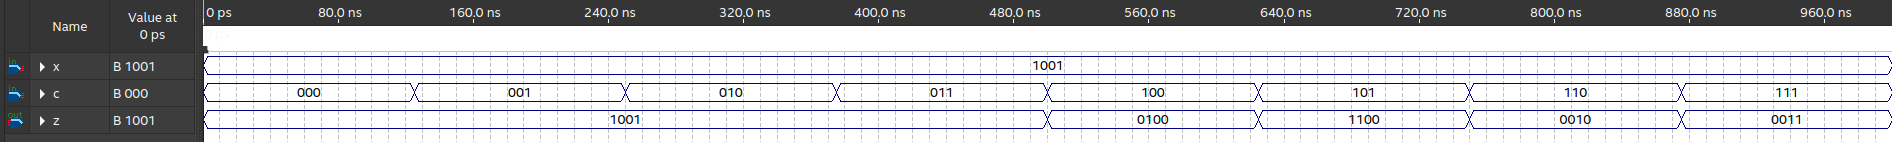
\includegraphics[width=\textwidth]{inciso-c-sim}
  \caption{Simulación del circuito (Parte C)}
  \label{fig:inciso_c_sim}
\end{figure}

Lo cual coincide con lo establecido en la Tabla \ref{tab:previo1_func}. Uno de 
los aspectos importantes de mencionar es que para la primera mitad del 
funcionamiento no altera la salida (tal como se estableció en el planteamiento 
de la actividad). De ahí en fuera, los demás casos son:
\begin{itemize}
  \item \textbf{Para \texttt{100}:} Se tiene un desplazador a la derecha.
  \item \textbf{Para \texttt{101}:} Se tiene un rotador a la derecha.
  \item \textbf{Para \texttt{110}:} Se tiene un desplazador a la izquierda.
  \item \textbf{Para \texttt{111}:} Se tiene un rotador a la izquierda.
\end{itemize}

Con lo cual queda comprobado el funcionamiento del circuito propuesto.

\end{document}

